\section{Простые утверждения}

\subsection{Основные тождества про теоретико-множественные операции, декартово произведение, возведение множества в степень множества.}

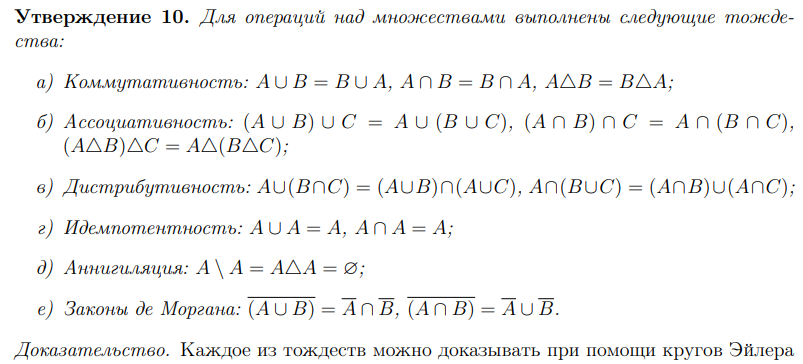
\includegraphics[width = 0.92\textwidth]{images/prop_10_sets.png}

\textbf{Определение:} Множества $A$ и $B$ эквивалентны, если для каждого элемента $A$ есть элемент $B$, задающий тот же кортеж, и наоборот. Будем обозначать такую эквивалентность как $A \sim B$.

\textbf{Cвойства:}
\begin{enumerate}
     \item $A^n \sim A\times A\ldots \times A$ -- по определению.
     \item $(A\times B)\times C \sim A \times( B \times C )$:\\
     $A \times B = \{(a,b): \ a \in A, b\in B\}; \\ (A \times B)\times C = \{((a,b),c): \ a \in A, b\in B, c \in C\} \sim \{(a,(b,c)): \ a \in A, b\in B, c \in C\} = A\times (B \times C)$.
     \item $A \times \{\emptyset\} \sim A$.
     \item $A^{n+k} \sim (\underbrace{A\times A \times \ldots \times A}_{n})(\underbrace{A\times A \times \ldots \times A}_{k}) \sim \underbrace{A\times A \times \ldots \times A}_{n+k} \sim A^n \times A^k$.
     \item $(A^n)^m \sim A^{nm}$.
\end{enumerate}

\textbf{Cвойства:}
\begin{enumerate}
    \item $(A \times B)^C \sim A^C \times B^C$.
    \item $A^{B \cup C} \sim A^B \times A^C$, если $B$ и $C$ не пересекаются.
    \item $(A^B)^C \sim A^{B \times C}$.
\end{enumerate}

\textit{Доказательство:} 
\begin{enumerate}
    \item Пусть $F \in (A \times B)^C$. Это значит, что $F : C \to A \times B$. То есть каждому элементу $c \in C$ сопоставлена некоторая пара $(a, b) \in A \times B$. Вместо этого ему можно сопоставить отдельно элементы $a \in A$ и $b \in B$. Получится два отображения, первое отображает $c$ в $a$, а второе -- $c$ в $b$, то есть пара отображений $(F_1, F_2) \in A^C \times B^C$.
    \item Вторая эквивалентность означает, что определить функцию на несвязном объединении двух множеств это то же самое, что определить её на каждом из этих множеств по отдельности.
    \item Третья эквивалентность означает, что функция двух аргументов есть то же самое, что отображение первого аргумента в функцию, зависящую от второго аргумента.
\end{enumerate}

\subsection{Равномощность — отношение эквивалентности.}

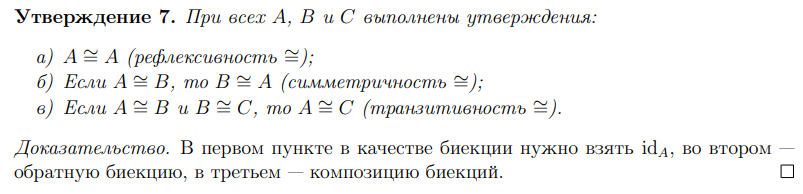
\includegraphics[width = 0.92\textwidth]{images/equiv_sets.png}

\subsection{Объединение и декартово произведение счётных множеств счётны.}

\textbf{Утверждение:} Пусть $A$ -- счётное множество, а $b \not\in A$. Тогда $A \cup \{b\}$ тоже счётно.

\textit{Доказательство:} Формально, пусть $\alpha: \N \to A$ -- биекция. Тогда определим биекцию $\beta: \N \to (A \cup \{b\})$ так: $\beta(0) = b$ и $\beta(n) = \alpha(n - 1)$ для $n > 0$.

\textbf{Утверждение:} Если $A$ счётно, а $B$ конечно, то $A \cup B$ тоже счётно.

\textbf{Утверждение:} Если $A$ и $B$ суть счётные множества, то $A \cup B$ тоже счётно.

\textit{Доказательство:} Ясно, что $A \cup B = A \cup (B \setminus A)$. Если множество $B \setminus A$ конечно, то утверждение следует из предыдущего. Иначе $B \setminus A$ счётно.

Таким образом, утверждение достаточно доказать для непересекающихся $A$ и $B$. В этом случае пусть $\alpha: \N \to A$ и $\beta : \N \to B$ суть биекции. Тогда построим биекцию $\gamma : \N \to A \cup B$ по правилу: $\gamma(2k) = \alpha(k)$, а $\gamma(2k + 1) = \beta(k)$.
    
\textbf{Утверждение:} Декартово произведение двух счётных множеств $A \times B$ cчётно.

\textit{Доказательство:} В самом деле, по определению декартово произведение есть множество всех упорядоченных пар вида $\langle a, b \rangle$, в которых $a \in A$ и $b \in B$. Разделим пары на группы, объединив пары с одинаковой первой компонентой (каждая группа имеет вид $\{a\}\times B$ для какого-то $a \in A$). Тогда каждая группа счётна, поскольку находится во взаимно однозначном соответствии с $B$ (пара определяется своим вторым элементом), и групп столько же, сколько элементов в $A$, то есть счётное число.

\subsection{В любом бесконечном множестве найдётся счётное подмножество.}
Так как $A$ бесконечно, в нем существует элемент $a_0$, причем $A\backslash{a_0}$ также бесконечно. Значит, в нем найдется $a_1$. Продолжая набирать элементы, получим множество $A_1 = \{a_0, a_1,\ldots\}$, $A_1 \subset A$.

\subsection{Несчётность множества точек на отрезке.}

Ясно, что любые два отрезка равномощны, так что рассмотрим отрезок $[0, 1]$. Докажем несчётность интервала $(0, 1)$, из чего будет несчётность отрезка.

Рассмотрим биекцию $f(x) = \tg(\pi(x - \frac{1}{2}))$.

\subsection{Нефундированность прямого лексикографического порядка на конечных словах.}
Нефундированность следует из существования бесконечно убывающей цепочки. Например, можно рассмотреть последовательность: $b > ab > aab > \ldots$.

\subsection{Любой начальный отрезок вполне упорядоченного множества, отличный от всего множества, представляется в виде $[0, a)$.}

\textbf{Теорема:} Если $S$ -- ВУМ, $A$ -- начальный отрезок $S$, $A \neq S$, то $A = [0, y)$.

\begin{proof}
    Рассмотрим $\overline{A} = S \backslash A$. Так как $\overline{A} \neq \varnothing$, то по свойству фундированности $\exists y =$ min$\overline{A},$ тогда покажем, что $A = [0, y)$. $[0, y) \subset A,$ так как если $x \in [0, y)$ и $x \notin A,$ то $x < y$ и $x \in \overline{A} \Rightarrow y \neq$ min$\overline{A}$, противоречие. $A \subset [0, y),$ так как если $x \in A$ и $x \notin [0, y),$ то (поскольку это ЛУМ) $x \geqslant y \Rightarrow$ (по определению начального отрезка) получаем, что $y \in A$ противоречие.
\end{proof}

\subsection{Вполне упорядоченное множество неизоморфно своему начальному отрезку вида
[0, a) (вывод из леммы о монотонной функции).}
\begin{center}
    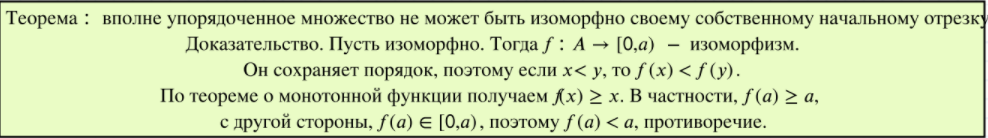
\includegraphics[width = 17cm]{images/2 (определения)_m211.PNG}
\end{center}

\subsection{Сумма и произведение фундированных множеств фундированы, вполне упорядоченных — вполне упорядочены.}

\begin{center}
    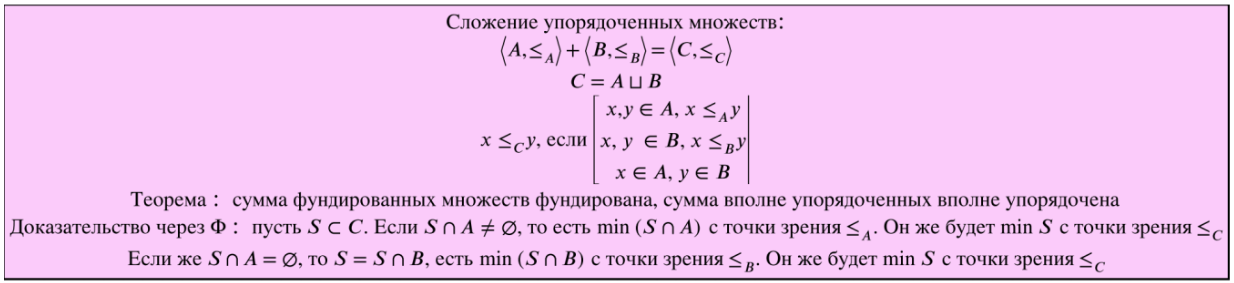
\includegraphics[width = 17cm]{images/sum_fund.png}
\end{center}
\begin{center}
    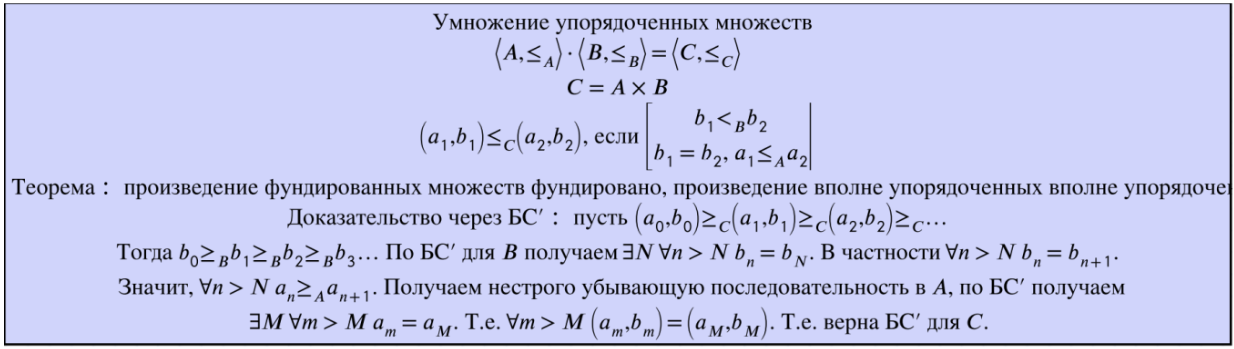
\includegraphics[width = 17cm]{images/cdot_fund.png}
\end{center}

\subsection{Свойства сложения и умножения вполне упорядоченных множеств: ассоциативность, некоммутативность, (не)дистрибутивность, (не)монотонность.}

Верны ассоциативность и правая дистрибутивность: $A\cdot(B + C) \simeq A\cdot B + A\cdot C$. Коммутативность и левая дистрибутивность неверны: $1+\omega = \omega \neq \omega+1$, $2 \cdot \omega = \omega \neq \omega \cdot 2$, $(1 + 1) \cdot \omega = \omega \neq 1 \cdot \omega + 1 \cdot \omega$.

Условие монотонности звучит так: если $A < B (A \lesssim B)$, то верно ли, что для всех $C$ истинно $A+C < B+C$, $C + A < C + B$, $A \cdot C < B \cdot C$, $C \cdot A < C \cdot B$ (то же для $\lesssim$ вместо $<$)?

При $A < B$ верно $C + A < C + B$, $A + C \lesssim B + C$, $C \cdot A < C \cdot B$ (при непустом $C$), $A \cdot C \lesssim B \cdot C$. При $A \lesssim B$ все неравенства верны с $\lesssim$.

\subsection{Сравнимость любых двух множеств по мощности (вывод из теоремы Цермело и свойств вполне упорядоченных множеств).}
\begin{center}
    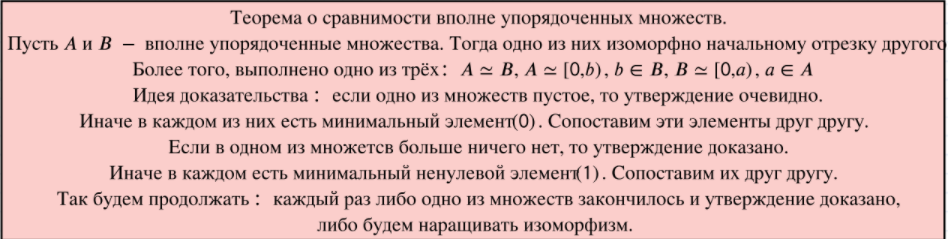
\includegraphics[width = 17cm]{images/2 (определения)_mm1.PNG}\\    
\end{center}
\textbf{Сравнимость любых двух множеств по мощности}\\
По теореме Цермело для любого множества существует равномощное ему ВУМ. Пусть даны $A, B$, а $A', B'$ соответствующие им ВУМы, удовлетворяющие теореме Цермело. Тогда из теоремы о сравнимости ВУМов $A'$ и $B'$ сравнимы по мощности, значит, $А$ и $В$ также сравнимы по мощности.

\subsection{Теорема о структуре: любой элемент вполне упорядоченного множества представляется как сумма предельного и конечного.}

\textbf{Теорема:} Для любого элемента $a$ вполне упорядоченного множества найдётся предельный элемент $b$ и натуральное число $k$, такое что $a = \underbrace{S(S(\ldots (S}_{k \text{ раз }}(b))\ldots))$.

\textit{Доказательство:} Нужно брать непосредственно предыдущий, пока не придём к предельному. Прийти обязаны, иначе будет бесконечно убывающая последовательность.